% Created by tikzDevice version 0.7.0 on 2015-04-28 20:16:18
% !TEX encoding = UTF-8 Unicode
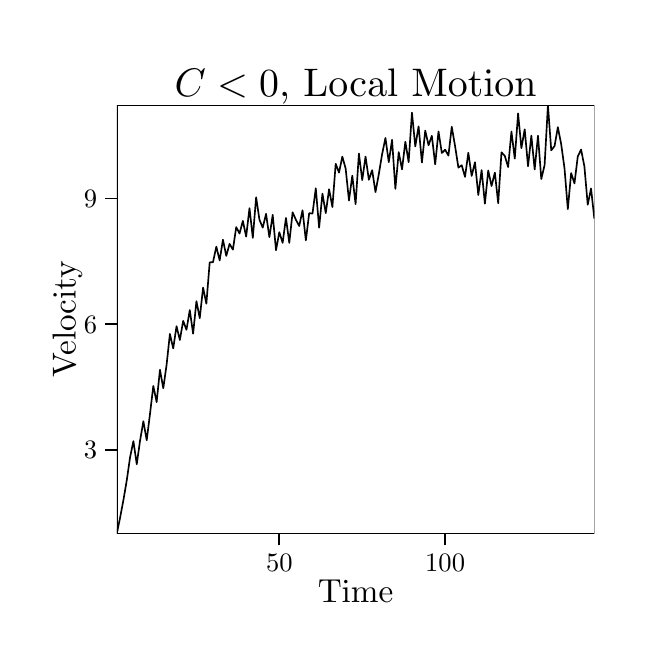
\begin{tikzpicture}[x=1pt,y=1pt]
\definecolor[named]{fillColor}{rgb}{1.00,1.00,1.00}
\path[use as bounding box,fill=fillColor,fill opacity=0.00] (0,0) rectangle (216.81,216.81);
\begin{scope}
\path[clip] (  0.00,  0.00) rectangle (216.81,216.81);
\definecolor[named]{drawColor}{rgb}{1.00,1.00,1.00}
\definecolor[named]{fillColor}{rgb}{1.00,1.00,1.00}

\path[draw=drawColor,line width= 0.6pt,line join=round,line cap=round,fill=fillColor] ( -0.00,  0.00) rectangle (216.81,216.81);
\end{scope}
\begin{scope}
\path[clip] ( 32.22, 34.03) rectangle (204.76,188.82);
\definecolor[named]{fillColor}{rgb}{1.00,1.00,1.00}

\path[fill=fillColor] ( 32.22, 34.03) rectangle (204.76,188.82);
\definecolor[named]{drawColor}{rgb}{0.00,0.00,0.00}

\path[draw=drawColor,line width= 0.6pt,line join=round] ( 32.22, 34.03) --
	( 33.42, 39.87) --
	( 34.62, 46.23) --
	( 35.82, 53.36) --
	( 37.01, 61.61) --
	( 38.21, 67.42) --
	( 39.41, 59.04) --
	( 40.61, 67.58) --
	( 41.81, 74.59) --
	( 43.01, 67.73) --
	( 44.20, 77.24) --
	( 45.40, 87.33) --
	( 46.60, 81.52) --
	( 47.80, 93.20) --
	( 49.00, 86.52) --
	( 50.19, 94.90) --
	( 51.39,106.13) --
	( 52.59,100.91) --
	( 53.79,108.93) --
	( 54.99,103.96) --
	( 56.19,110.86) --
	( 57.38,107.63) --
	( 58.58,114.77) --
	( 59.78,106.22) --
	( 60.98,117.97) --
	( 62.18,111.84) --
	( 63.38,122.87) --
	( 64.57,117.06) --
	( 65.77,132.00) --
	( 66.97,132.08) --
	( 68.17,137.69) --
	( 69.37,132.70) --
	( 70.56,140.20) --
	( 71.76,134.35) --
	( 72.96,138.68) --
	( 74.16,136.61) --
	( 75.36,144.74) --
	( 76.56,142.41) --
	( 77.75,146.99) --
	( 78.95,141.32) --
	( 80.15,151.60) --
	( 81.35,140.85) --
	( 82.55,155.52) --
	( 83.75,147.41) --
	( 84.94,144.55) --
	( 86.14,149.53) --
	( 87.34,141.10) --
	( 88.54,149.17) --
	( 89.74,136.41) --
	( 90.93,142.89) --
	( 92.13,139.06) --
	( 93.33,148.05) --
	( 94.53,139.05) --
	( 95.73,150.09) --
	( 96.93,147.38) --
	( 98.12,145.15) --
	( 99.32,150.81) --
	(100.52,139.95) --
	(101.72,149.78) --
	(102.92,149.64) --
	(104.11,158.77) --
	(105.31,144.53) --
	(106.51,156.85) --
	(107.71,149.80) --
	(108.91,158.43) --
	(110.11,152.00) --
	(111.30,167.63) --
	(112.50,164.43) --
	(113.70,170.22) --
	(114.90,165.89) --
	(116.10,154.37) --
	(117.30,163.33) --
	(118.49,153.03) --
	(119.69,171.34) --
	(120.89,161.72) --
	(122.09,170.22) --
	(123.29,161.86) --
	(124.48,165.32) --
	(125.68,157.39) --
	(126.88,163.86) --
	(128.08,171.13) --
	(129.28,176.94) --
	(130.48,168.22) --
	(131.67,176.28) --
	(132.87,158.57) --
	(134.07,171.82) --
	(135.27,165.62) --
	(136.47,175.58) --
	(137.66,168.22) --
	(138.86,186.10) --
	(140.06,173.90) --
	(141.26,181.15) --
	(142.46,168.09) --
	(143.66,179.62) --
	(144.85,174.34) --
	(146.05,177.74) --
	(147.25,167.41) --
	(148.45,179.32) --
	(149.65,171.52) --
	(150.85,172.71) --
	(152.04,170.57) --
	(153.24,181.00) --
	(154.44,174.01) --
	(155.64,166.24) --
	(156.84,167.09) --
	(158.03,162.89) --
	(159.23,171.60) --
	(160.43,163.23) --
	(161.63,168.17) --
	(162.83,156.36) --
	(164.03,165.32) --
	(165.22,153.20) --
	(166.42,165.21) --
	(167.62,159.61) --
	(168.82,164.45) --
	(170.02,153.37) --
	(171.21,171.76) --
	(172.41,170.47) --
	(173.61,166.44) --
	(174.81,179.27) --
	(176.01,169.49) --
	(177.21,185.81) --
	(178.40,173.26) --
	(179.60,180.07) --
	(180.80,166.73) --
	(182.00,177.79) --
	(183.20,165.57) --
	(184.40,177.79) --
	(185.59,162.12) --
	(186.79,167.15) --
	(187.99,188.82) --
	(189.19,172.48) --
	(190.39,174.04) --
	(191.58,180.84) --
	(192.78,174.73) --
	(193.98,166.02) --
	(195.18,151.24) --
	(196.38,164.27) --
	(197.58,160.54) --
	(198.77,170.22) --
	(199.97,172.77) --
	(201.17,166.68) --
	(202.37,152.84) --
	(203.57,158.69) --
	(204.76,147.84);

\path[draw=drawColor,line width= 0.6pt,line join=round,line cap=round] ( 32.22, 34.03) rectangle (204.76,188.82);
\end{scope}
\begin{scope}
\path[clip] (  0.00,  0.00) rectangle (216.81,216.81);
\definecolor[named]{drawColor}{rgb}{0.00,0.00,0.00}

\node[text=drawColor,anchor=base east,inner sep=0pt, outer sep=0pt, scale=  0.96] at ( 25.11, 60.98) {3};

\node[text=drawColor,anchor=base east,inner sep=0pt, outer sep=0pt, scale=  0.96] at ( 25.11,106.38) {6};

\node[text=drawColor,anchor=base east,inner sep=0pt, outer sep=0pt, scale=  0.96] at ( 25.11,151.78) {9};
\end{scope}
\begin{scope}
\path[clip] (  0.00,  0.00) rectangle (216.81,216.81);
\definecolor[named]{drawColor}{rgb}{0.00,0.00,0.00}

\path[draw=drawColor,line width= 0.6pt,line join=round] ( 27.95, 64.28) --
	( 32.22, 64.28);

\path[draw=drawColor,line width= 0.6pt,line join=round] ( 27.95,109.69) --
	( 32.22,109.69);

\path[draw=drawColor,line width= 0.6pt,line join=round] ( 27.95,155.09) --
	( 32.22,155.09);
\end{scope}
\begin{scope}
\path[clip] (  0.00,  0.00) rectangle (216.81,216.81);
\definecolor[named]{drawColor}{rgb}{0.00,0.00,0.00}

\path[draw=drawColor,line width= 0.6pt,line join=round] ( 90.93, 29.77) --
	( 90.93, 34.03);

\path[draw=drawColor,line width= 0.6pt,line join=round] (150.85, 29.77) --
	(150.85, 34.03);
\end{scope}
\begin{scope}
\path[clip] (  0.00,  0.00) rectangle (216.81,216.81);
\definecolor[named]{drawColor}{rgb}{0.00,0.00,0.00}

\node[text=drawColor,anchor=base,inner sep=0pt, outer sep=0pt, scale=  0.96] at ( 90.93, 20.31) {50};

\node[text=drawColor,anchor=base,inner sep=0pt, outer sep=0pt, scale=  0.96] at (150.85, 20.31) {100};
\end{scope}
\begin{scope}
\path[clip] (  0.00,  0.00) rectangle (216.81,216.81);
\definecolor[named]{drawColor}{rgb}{0.00,0.00,0.00}

\node[text=drawColor,anchor=base,inner sep=0pt, outer sep=0pt, scale=  1.20] at (118.49,  9.03) {Time};
\end{scope}
\begin{scope}
\path[clip] (  0.00,  0.00) rectangle (216.81,216.81);
\definecolor[named]{drawColor}{rgb}{0.00,0.00,0.00}

\node[text=drawColor,rotate= 90.00,anchor=base,inner sep=0pt, outer sep=0pt, scale=  1.20] at ( 17.30,111.43) {Velocity};
\end{scope}
\begin{scope}
\path[clip] (  0.00,  0.00) rectangle (216.81,216.81);
\definecolor[named]{drawColor}{rgb}{0.00,0.00,0.00}

\node[text=drawColor,anchor=base,inner sep=0pt, outer sep=0pt, scale=  1.44] at (118.49,191.84) {$C < 0$, Local Motion};
\end{scope}
\end{tikzpicture}
